\chapter{Développement d'une méthode d'angiographie dynamique avec une séquence d'imagerie radiale à encodage pseudo-aléatoire par un double angle d'or ciné.}
\setlength{\footskip}{50pt}
\chaptermark{Angiographie dynamique avec double angle d'or}

\label{Chap3}
\section{Contexte}

Dans de nombreuses pathologies vasculaires, l’intégrité physique du vaisseau est touchée. Afin de visualiser les vaisseaux de manière non invasive, l’Angiographie par Résonance Magnétique (ARM) est devenue une technique de référence en clinique. Elle permet en effet d’apprécier l’anatomie des vaisseaux et visualiser les déformations de ces derniers (sténose, anévrisme, …). Néanmoins, dans de nombreuses pathologies, ou dans le cas d’un diagnostic précoce, l’imagerie anatomique n’est pas un examen suffisant et les informations obtenues apparaissent normales. Il apparaît donc intéressant de développer des méthodes d'investigation fonctionnelles, permettant de visualiser et quantifier le flux sanguin dans les vaisseaux. Pour obtenir ces informations, il est nécessaire de recueillir des images à la fois en trois dimensions et résolues dans le temps. On parle alors d’angiographie 4D.

Les problématiques que l'on peut rencontrer chez le petit animal ne sont pas les mêmes que chez l'humain ce qui limite l'utilisation de certaines séquences ou nécessite une adaptation. L'une des limitations principales pour effectuer la mesure de flux chez la souris est son rythme cardiaque supérieur à 400 battements par minutes lorsque celle-ci est anesthésiée. La résolution temporelle de la séquence doit dont être importante pour obtenir une bonne visualisation de la dynamique des flux. Afin d’apprécier la vitesse du sang dans les vaisseaux plusieurs méthodes sont disponibles en IRM chez l’homme : 
\begin{itemize}
\item L’imagerie de prise de contraste du Gadolinium. Pour cette technique, les acquisitions sont faites assez rapidement pour visualiser l’arrivée du produit dans lez zones d’intérêt. Aujourd’hui, avec les progrès instrumentaux et méthodologiques, il est possible d’obtenir des images sub-millimétriques en moins d’une seconde \cite{Wu:2011ys}. Ces méthodes sont aujourd’hui les méthodes de référence chez l’homme. En revanche, leurs transferts chez le petit animal apparaît difficile voir impossible compte tenu de la taille des vaisseaux observés et de la cinétique de biodistribution des agents de contraste (moins de 2 secondes pour le premier passage d’un agent de contraste classique à base de Gadolinium).

\item L’imagerie 4D par contraste de phase \cite{Markl:2012pi}. Cette méthode est aujourd’hui de plus en plus répandue en clinique et a permis d’étudier de nombreuses pathologies comme les complications après la réparation d'un anévrisme ou d'une dissection de l'aorte \cite{frydrychowicz2011aortic} , des pathologies associées aux remplacements des valves aortiques \cite{kvitting2004flow} ou bien pour étudier l'hypertension pulmonaire artérielle \cite{sanz2007pulmonary}.
Grâce à l’application d’un gradient bipolaire de durée et d’intensité déterminées, le déphasage des spins est alors proportionnel à la vitesse du flux. Cette méthode a pour principal avantage d’offrir une visualisation de la vitesse et de la direction du flux voxel par voxel. Toutefois, l’inconvénient majeur de cette technique est son temps d’acquisition long puisqu’il est nécessaire de répéter la séquence 4 fois pour encoder la vitesse dans toutes les directions \cite{Johnson:2010uq,Robson:2010uq,Wu:2013ys}. 
Chez le petit animal, une fois de plus, compte tenu de la taille des zones à observer, du manque de rapport signal-sur-bruit, ce type d’acquisition de mesure des flux est peu répandu. En imagerie 2D seules quelques publications ont montré le potentiel de la méthode, et à notre connaissance en imagerie 3D+t, seule une publication est rapportée \cite{Janiczek:2011qm}.

\item L’imagerie par marquage de spin. Cette méthode permet d’estimer la vitesse des flux grâce à des acquisitions multiples avec ou sans marquage des spins sanguins puis une soustraction des images obtenues (Koktzoglou and Edelman \cite{Koktzoglou:2009fe}). Le desavantage de cette méthode est qu’elle necessite deux acquisitions, donc un temps d’acquisition relativement important.
Une méthode alternative basée sur l’imagerie ciné temps-de-vol (Time-Of-Flight : TOF) a été développée au sein du laboratoire par  Miraux et al. \cite{Miraux:2006fu} et appliquée chez le petit animal. Celle-ci consiste, après la détection d’un pic ECG, à saturer le signal dans le volume d'imagerie puis à recueillir le signal du sang frais progressant dans les vaisseaux (voir figure \ref{fig:SeqSylvain}) à l’aide de séquences ciné 3D.
\end{itemize}

\begin{figure}[H]
\centering
\line(1,0){400} \\
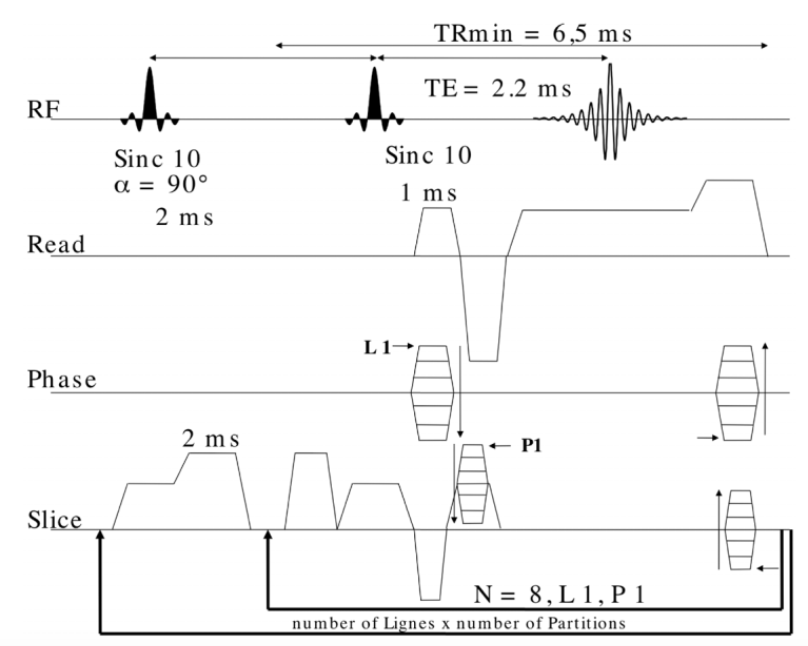
\includegraphics[scale=0.5]{./figure/chap3/SeqSylvain.png}
\caption[Séquence d'angiographie dynamique.]{\label{fig:SeqSylvain} \textbf{Séquence d'angiographie dynamique.} Chronogramme de la séquence utilisée pour obtenir une ARM "sang-blanc" résolue dans le temps. L = Nombre de ligne, P = Nombre de partition, N = Nombre d'images résolues dans le temps. (Figure extraite de Miraux et al. 2006 \cite{Miraux:2006fu})}
\line(1,0){400} \\ \end{figure}

La méthode d'imagerie de flux par temps-de-vol a permis de mesurer les flux sanguins dans diverses artères chez la souris : carotides \cite{Miraux:2006fu}, pulmonaires \cite{Cochet:2013dk} et même coronaires \cite{Cochet:2010ec} ainsi que dans le polygone de Willis.

Néanmoins, le temps d’acquisition pour cette angiographie ciné 3D reste long, en particulier lorsqu’il est nécessaire d’obtenir des images avec des résolutions spatiale et temporelle élevées. Pour réduire ces temps d’acquisition, les techniques d’imagerie parallèle peuvent être utilisées mais avec le matériel disponible en imagerie préclinique, un gain maximum d’un facteur 2 peut être atteint et ceci au détriment du rapport signal-sur-bruit. 

C’est pourquoi, il a été choisi de s'orienter vers une autre stratégie afin de diminuer les temps d’acquisition de manière significative. Cette stratégie se base sur les techniques d’acquisition radiale parce qu’elles permettent en théorie d’obtenir de forts facteurs de sous-échantillonnage. Elles sont également extrêmement flexibles et adaptables aux méthodes de rehaussement de résolution spatiale de type fenêtre glissante.

Le but des travaux présentés dans ce chapitre est donc de combiner la méthode d’angiographie dynamique par temps-de-vol avec des trajectoires 3D radiales afin de générer des images à fortes résolutions spatiale et temporelle rapidement. Pour cela nous avons mis au point une méthode originale d’encodage doublement pseudo-aléatoire.


\section{Angiographie à partir de séquence radiale.}

L'un des inconvénients de la trajectoire cartésienne est son manque de flexibilité dans la reconstruction de l'image. Une fois que la résolution temporelle a été déterminée par le nombre de lignes successives à recueillir pour chaque répétition, il est difficile d'obtenir des images de bonne qualité (à partir du même jeu de donnée) avec une résolution temporelle différente.
Les trajectoires radiales sont plus flexibles car elles permettent de reconstruire des images intermédiaires sans attendre d'avoir recueilli toutes les projections de l'espace de Fourier. Mais, comme montré dans la figure \ref{fig:SousEchan}, cela est très dépendant de la méthode de répartition des projections qui est employée. La répartition linéaire permet d'obtenir une répartition homogène des projections lorsque toutes les données sont recueillies mais elle manque de flexibilité lors de la reconstruction d'une image n'utilisant seulement qu'une partie des données recueillies durant un temps donné. Il est donc nécessaire de proposer des répartitions pseudo-aléatoires qui permettront de répartir de manière plus homogène les projections au cours du temps et donc d'obtenir des images de meilleure qualité par exemple dans la figure \ref{fig:SousEchan}.droite.

De nombreuses méthodes de répartition pseudo-aléatoire des projections 2D et 3D ont été étudiées : les méthodes utilisant des trajectoires multi-spirales \cite{Chan:2009uq}, la méthode quasi-"random" \cite{Tibiletti2015Multistage-thre}, les méthodes d'inversion de bit \cite{Theilmann2004View-ordering-i}, les séquences Halton \cite{chan2009halton} ou bien encore des méthodes utilisant l'angle d'or \cite{Winkelmann:2007fk}. Winkelmann et al. \cite{Winkelmann:2007fk} et Song et al. \cite{Song:2000fk} ont montré que l'imagerie radiale 2D est plus flexible en utilisant un angle d'or, dérivé du facteur d'or (décrit dans la prochaine section). Par exemple en imagerie de prise de contraste dynamique, en positionnant les projections dans l'espace de Fourier avec cet angle, il est possible à partir de n'importe quelle position de reconstruire une image. Le nombre de projections à utiliser peut être adapté à la résolution spatio-temporelle souhaitée. Chan et al. \cite{Chan:2009uq} ont montré qu'il était possible d'étendre la notion d'angle d'or à l'imagerie radiale 3D et ont montré son application à l'imagerie dynamique de prise de contraste dans les tumeurs du sein.

La méthode se basant sur l’angle d’or a été privilégiée dans les travaux montrés ici.

\begin{figure}[H]
\centering
\line(1,0){400} \\
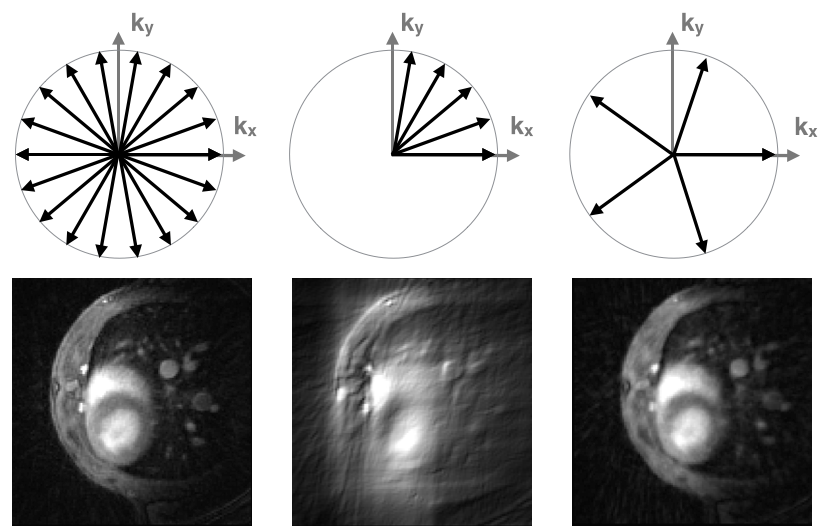
\includegraphics[scale=0.5]{./figure/chap3/SousEchan.png}
\caption[Homogénéité de répartition des projections.]{\label{fig:SousEchan} \textbf{Homogénéité de répartition des projections.} Vues axiales obtenues avec une séquence UTE 2D sur le coeur de souris en fonction de la répartition des projections dans l'espace de Fourier. A gauche : l'image est reconstruite avec les 402 projections réparties de façon homogène dans l'espace de Fourier pour atteindre le critère de Nyquist. Au centre : l'image est acquises avec 100 projections réparties de manière adjacente. A droite : l'image est reconstruite avec 100 projections réparties de manière uniforme sur le plan.}
\line(1,0){400} \\ \end{figure}

\subsection{Angle d'or}

L'angle d'or $\phi$ est dérivé du facteur d'or qui est extrait de la suite de Fibonacci. Il est utilisé en IRM pour de nombreuses applications permettant de répartir au mieux des données dans l'espace de Fourier. En imagerie radiale 2D, cet angle d'or $\phi$ est égale à $111,24 \degres$. Chaque projection est donc séparée de la précédente par cet angle $\phi$. Cela a pour effet de bien répartir spatialement et temporellement les projections au cours du temps (figure \ref{fig:Gold2D})

\begin{figure}[H]
\centering \line(1,0){400} \\
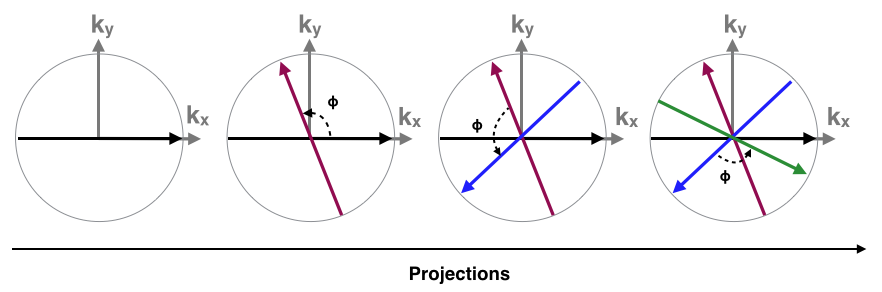
\includegraphics[scale=0.6]{./figure/chap3/Gold2D.png}
\caption[Angle d'or 2D.]{\label{fig:Gold2D} \textbf{Angle d'or 2D.} Schéma de l'ordre d'acquisition des projections radiales dans l'espace de Fourier basé sur l'angle d'or 2D.}
\line(1,0){400} \\ \end{figure}

\begin{figure}[H]
\centering \line(1,0){400} \\
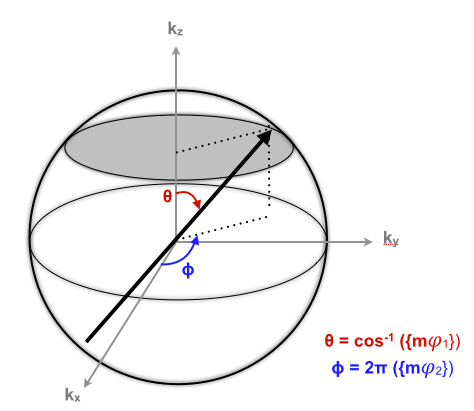
\includegraphics[scale=0.4]{./figure/chap3/Gold3D.png}
\caption[Angle d'or 3D.]{\label{fig:Gold3D} \textbf{Angle d'or 3D.} Positionnement des projections radiales dans l'espace de Fourier basé sur l'angle d'or 3D où m est le numéro de la projection.}
\line(1,0){400} \\ \end{figure}

Ce principe d'angle d'or a été étendu à l'imagerie 3D. Deux facteurs d'or sont nécessaires à son implémentation ($\phi_1=0,4656$; $\phi_2=0,6823$). Ici, la méthode de répartition des projections employée pour l'imagerie 3D utilise $\phi_1$ pour orienter la projection d'un angle $\phi$ par rapport à l'axe $k_z$ et $\phi_2$ pour déterminer l'angle polaire $\theta$ de la projection dans le plan $(k_x,k_y)$ (figure \ref{fig:Gold3D}) selon les équations suivantes :
\begin{equation}
\label{eq:GoldPremier}
\begin{array}{c}
\Phi_i=2\pi \times mod(\phi_1 \times i,1) \\
\theta_i=2 \times acos(mod(\phi_2 \times i,1)) -1
\end{array}
\end{equation}
où i est le numéro de la projection. Comme montré dans la figure \ref{fig:ComparTraj}, on observe que la répartition des projections au cours du temps est uniforme dans l'espace.

\begin{figure}[h]
\centering \line(1,0){400} \\
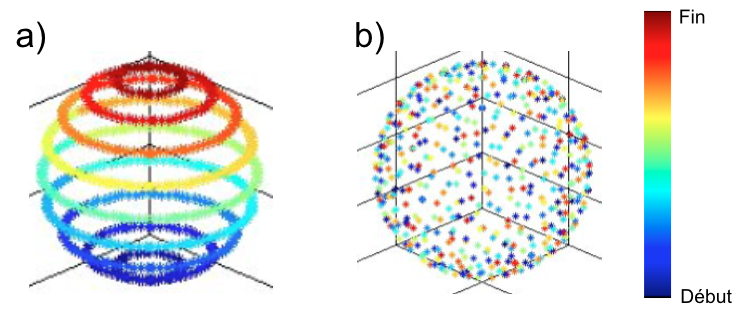
\includegraphics[scale=0.4]{./figure/chap3/ComparTraj.png}
\caption[Comparaison du positionnement des projections au cours du temps.]{\label{fig:ComparTraj} \textbf{Comparaison du positionnement des projections au cours du temps.} Positionnement des derniers points de chaque projection radiale dans l'espace de Fourier au cours du temps selon les méthodes : (a) utilisée sur les imageurs Brüker (b) basée sur l'angle d'or 3D.}
\line(1,0){400} \\ \end{figure}

\subsection{Angiographie anatomique avec l'angle d'or et sous-échantillonnage}

Des images d'angiographie temps-de-vol au niveau des carotides de plusieurs souris ont été acquises avec une séquence d'imagerie radiale 3D et une répartition des projections à l'aide de l'angle d'or. Le nombre de projections utilisé au départ (40 000) pour reconstruire les images a ensuite été réduit à 8 000, 4 000 et 2 500. Ces images ont été comparées qualitativement à une image obtenue avec un encodage cartésien.

\begin{figure}[H]
\centering \line(1,0){400} \\
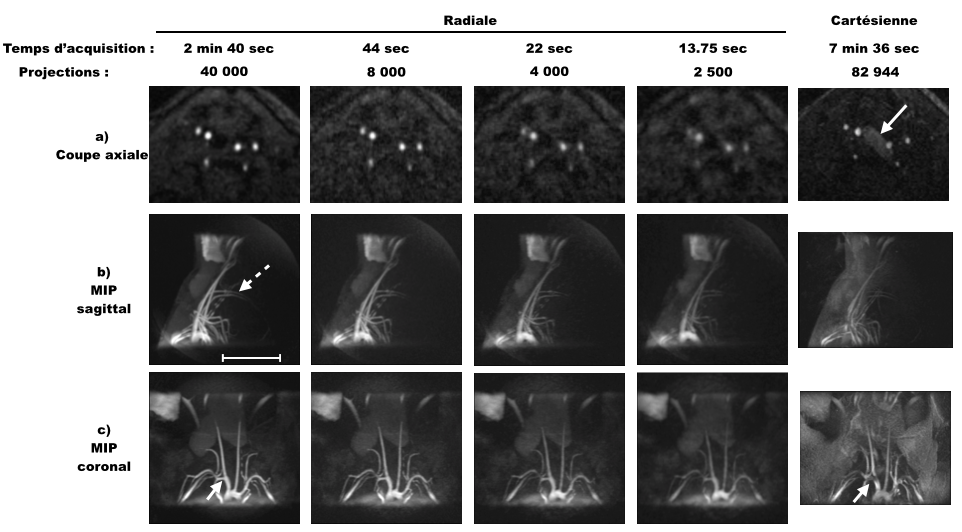
\includegraphics[scale=0.5]{./figure/chap3/RadialAnat.png}
\caption[Sous-échantillonnage en imagerie radiale 3D avec l'angle d'or 3D.]{\label{fig:RadialAnat} \textbf{Sous-échantillonnage en imagerie radiale 3D avec l'angle d'or 3D.}  Coupe axiale et projections d'intensité maximale (sagittale et coronale) issues d'une imagerie anatomique 3D positionnée au niveau des carotides d'une souris en acquisition radiale et cartésienne. Le nombre de projections utilisées en méthode radiale est de 40 000, 8 000, 4 000 et 2 500 projections. La barre d'échelle correspond à une longueur de 10 mm. }
\line(1,0){400} \\ 
\end{figure}

Comme on peut le voir sur la figure \ref{fig:RadialAnat}, malgré des facteurs de sous échantillonnage importants en imagerie radiale (5, 10, 16) la plupart des gros vaisseaux sont visibles sur les images avec aussi bien 8 000, 4 000 que 2 500 projections. Néanmoins, l’effet du fort sous-échantillonnage se traduit par une difficulté à distinguer les parties des artères les plus petites en taille sur les images d’intensité de projection maximale (MIP) comme indiqué par la flèche en pointillé. Cependant, l’angiogramme complet est bien défini avec seulement 4 000 projections correspondant à un temps d’acquisition de 22 secondes. 
Sur les images recueillies avec la séquence cartésienne, en dépit d’un temps d’acquisition beaucoup plus élevé, de nombreux artefacts sont observés. On distingue en effet la présence du repliement de la crosse aortique provoqué par un artefact de flux sur l’image axiale qui n’est pas présent en imagerie radiale. Le signal du sang apparaît moins important et moins homogène que sur les images radiales en particulier au niveau des flux turbulents comme montré par la petite flèche blanche.
L’acquisition de ces images anatomiques a permis de montrer la robustesse aux artefacts de flux et de mouvement des séquences radiales en comparaison avec les séquences cartésiennes.  
L’utilisation de l’angle d’or 3D permet de répartir l’information uniformément en fonction du temps dans l’espace de Fourier et ainsi obtenir des images de qualité dans un temps restreint.

\section{Angiographie radiale résolue dans le temps.}

\subsection{Séquence}

La séquence d’imagerie radiale utilisée pour la visualisation du flux chez le petit animal est montrée en figure \ref{fig:SeqARMAurel}. Elle est basée sur la séquence publiée en 2006 par Miraux et al. \cite{Miraux:2006fu}. Elle est constituée, en amont, d'un module de saturation sélectif du volume d'imagerie. Après ce module, une séquence d'écho de gradient 3D rapide est appliquée et répétée un nombre de fois N correspondant au nombre d'images ciné que l'on souhaite reconstruire. Cette séquence d'écho de gradient est constituée d'une impulsion radiofréquence sélective dans l'espace permettant d'obtenir un signal temps-de-vol dans le volume imagé. L'impulsion radiofréquence est suivie d'un gradient de rephasage de coupe combiné à des gradients de déphasage selon les trois axes permettant de se déplacer vers l'extérieur de l'espace de Fourier. Les gradients sont ensuite inversés pour permettre la lecture du signal selon une projection donnée. 
L'intensité des gradients sur les axes x, y et z est modulée en fonction du numéro de la trajectoire à recueillir, ici noté i, et déterminée grâce à un calcul préalable des coordonnées $kx_i$, $ky_i$ et $kz_i$ du point de départ de la projection. Ces coordonnées sont données par les équations suivantes :
\begin{equation}
\label{eq:GoldSecond}
\begin{array}{c}
kx_i = kmax \times \cos(\Phi_i) \sin(\theta_i) \\
ky_i = kmax \times \sin(\Phi_i) \sin(\theta_i) \\
kz_i = kmax \times \cos(\theta_i)
\end{array}
\end{equation}
où $\Phi_i$ et $\theta_i$ sont obtenues grâce à l'équation \ref{eq:GoldPremier} définissant les trajectoires selon l'angle d'or 3D. Des gradients de "spoiling" sont ensuite appliqués pour déphaser le signal résiduel à chaque TR.

\begin{figure}[H]
\centering \line(1,0){400} \\
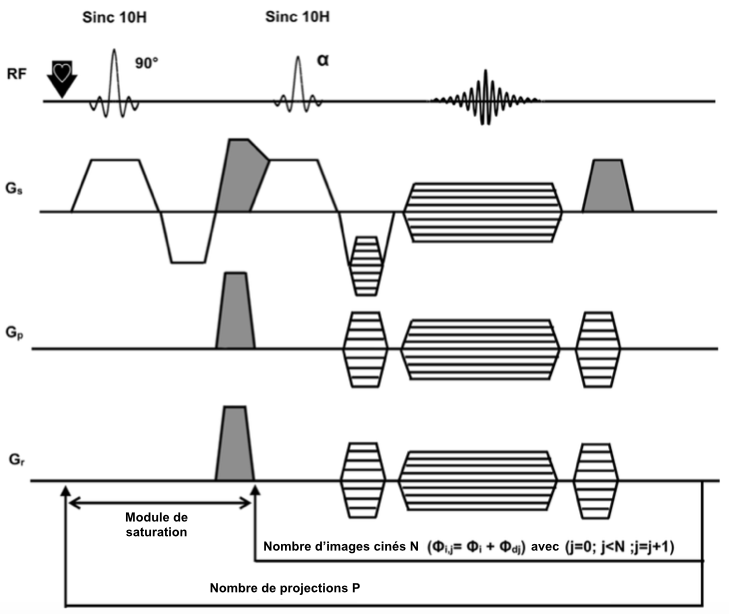
\includegraphics[scale=0.5]{./figure/chap3/SeqARMAurel.png}
\caption[Chronogramme de la séquence ARM sang blanc 3D+t radiale synchronisée sur l'ECG.]{\label{fig:SeqARMAurel}\textbf{ Chronogramme de la séquence ARM sang blanc 3D radiale synchronisée sur l'ECG.} Un module de saturation a été ajouté avant l'acquisition de N images ciné. Chacune de ces images a été acquise avec P projections. Pour chaque image ciné, $\Phi_{i,j} = \Phi_i+\Phi d_j$, où i est le nombre de projection et j est le nombre de ciné. Les gradients de déphasage sont indiqués en gris. La flèche noire représente la synchronisation ECG.}
\line(1,0){400} \\ \end{figure}

\subsection{Second angle d'or}

Généralement en imagerie résolue dans le temps, N signaux IRM sont recueillis successivement avec la même trajectoire dans l'espace de Fourier. Cela est répété de manière à pouvoir remplir N espaces de Fourier complets afin de pouvoir reconstruire N images (souvent appelé image ciné). Lorsque les temps de répétition sont courts par rapport aux mouvements que l'on souhaite observer, la différence entre les images est très faible et l'on obtient donc une redondance importante dans les informations contenues dans l'espace de Fourier. Or, comme expliqué dans la section \ref{subsec:KSpaceRegion}, il est possible d'exploiter les hautes fréquences pour augmenter la résolution de l'image. Cependant la méthode standard d'imagerie résolue dans le temps ne permet pas de flexibilité spatiotemporelle entre les différentes images reconstruites. Ce manque de flexibilité est présent que l'on utilise des trajectoires cartésiennes ou non-cartésiennes car il provient seulement du fait que les trajectoires utilisées entre les images ciné sont les mêmes. Pour résoudre ce problème, il est donc nécessaire de modifier les trajectoires entre les images ciné de manière à pouvoir ensuite les manipuler par exemple en additionnant deux espaces de Fourier ce qui permet de gagner en résolution spatiale et en signal mais réduit la résolution temporelle. 

La méthode choisie a été de recueillir le signal de chaque moment du cycle cardiaque avec des trajectoires similaires mais subissant une rotation autour de l'axe $k_z$. L'angle employé, noté $\Phi d_j$ est aussi basé sur l'angle d'or 2D $v_2$ et s'intègre dans les équations précédentes de la manière suivante :
\begin{equation}
\begin{array}{c}
\Phi_i=2\pi \times mod(\phi_1 \times i,1) +\Phi d_j\\
\theta_i=acos(mod(\phi_2 \times i,1)) \\
avec\ \ \Phi d_j=2\pi \times  mod( v_2 \times j)
\end{array}
\end{equation}
où j correspond au numéro de l'espace de Fourier du cycle cardiaque qui sera complété par cette projection. Cette méthode permet donc d'obtenir une répartition similaire des projections mais avec des trajectoires d'échantillonnage différentes dans l'espace de Fourier (figure \ref{fig:GoldCine}) en fonction de la position dans le cycle cardiaque. Cette méthode est plus efficace qu'une simple rotation de la trajectoire d'un angle (360/Nombre d'images ciné) car, lors de la reconstruction, les espaces de Fourier ainsi recueillis seront très proches. Il est au contraire préférable d'avoir un angle plus élevé qui permettra d'obtenir des trajectoires très différentes sur les ciné adjacentes plutôt que des trajectoires proches qui donneront peu de nouvelles informations pour améliorer la résolution spatiale. 
L'implémentation de ces trajectoires dans une séquence d'ARM dynamique de flux est décrite dans la figure \ref{fig:SeqARMAurel} sous forme de chronogramme.
 
\begin{figure}[H]
\centering \line(1,0){400} \\
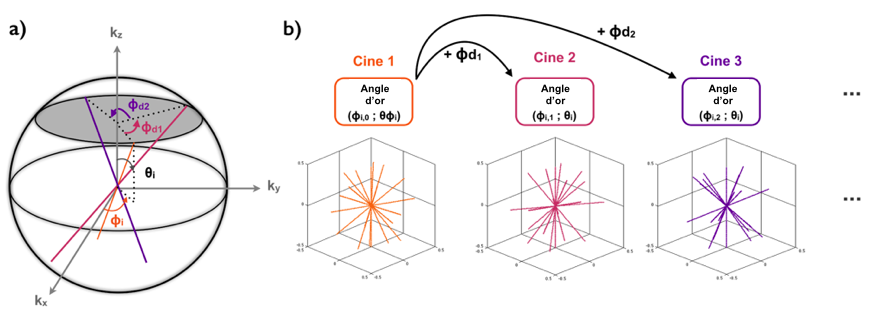
\includegraphics[scale=0.4]{./figure/chap3/GoldCine.png}
\caption[Répartition grâce à l'angle d'or entre les images ciné.]{\label{fig:GoldCine} \textbf{Répartition grâce à l'angle d'or entre les images ciné.} Description de la méthode utilisée pour obtenir une répartition différente des projections entre des images ciné consécutives. (a) Le segment orange représente la trajectoire d'une projection définie par le premier angle d'or, correspondant à l'image ciné 1 . Pour l'image ciné 2 (rose), la nouvelle trajectoire est obtenue en ajoutant l'angle $\Phi d_1$. Pour l'image ciné 3 (violet), l'angle ajouté est égale à $\Phi d_2$. La même valeur d'angle $\theta_i$, est utilisée entre les projections des images ciné adjacentes. (b) Exemple sur la distribution de 9 projections pour 3 images ciné consécutives.}
\line(1,0){400} \\ \end{figure}

\subsection{Filtre temporel}

Grâce à la méthode d’encodage doublement pseudo-aléatoire implantée, il est possible, \textit{a posteriori}, d’utiliser un filtre temporel pour reconstruire une image ciné à un temps donné du cycle cardiaque. Ce filtre temporel permet de regrouper les données de l'espace de Fourier que l'on veut reconstruire avec une partie des hautes fréquences des espaces de Fourier adjacents. De nombreux filtres différents peuvent être créés et adaptés \textit{a posteriori} lors de la reconstruction comme des filtres exponentiels ou linéaires qui s'utilisent pour des images de prises de contraste dynamiques \cite{Lin:2008uq}.
Il a ici été décidé d'utiliser un filtre défini par 2 paramètres, Q et R ($Q \leq R$) qui correspondent à des distances temporelles entre les espaces de Fourier dans le cycle cardiaque par rapport à l'espace de Fourier à reconstruire. Pour reconstruire l'image située à la position x du cycle cardiaque, tout l'espace de Fourier à cette position sera utilisé auquel sera ajouté la moitié des hautes fréquences des espaces situés à une position s tel que : $x-Q < s \leq x+Q$. Et enfin il sera également ajouté le quart des hautes fréquences des espaces de Fourier situés à une position $x-Q-R \leq s < x-Q$ et $x+Q \geq s \geq x+Q+R$. La forme de ce filtre est illustrée dans la figure \ref{fig:filtre} pour des valeurs R = 3 et Q = 1.
La résolution temporelle est donc étalée sur 7 TR mais le fait de ne pas utiliser les basses fréquences dans les images ciné adjacentes permet de réduire la résolution temporelle effective.
Après application du filtre temporel, on obtient un espace de Fourier que l'on peut exploiter avec la méthode de remaillage des données ("gridding") standard décrit dans le chapitre précédente.
L'utilisation d'un filtre temporel n'est pas uniforme sur tout le cycle cardiaque. En effet, des effets de bords réduiront la qualité des images que l'on peut obtenir au début et à la fin du cycle cardiaque.

\begin{figure}[H]
\centering \line(1,0){400} \\
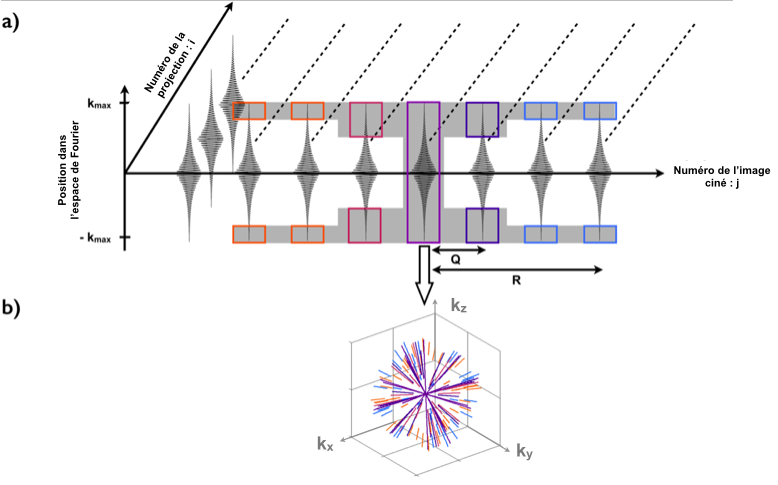
\includegraphics[scale=0.45]{./figure/chap3/filtre.png}
\caption[Exemple de filtre temporel.]{\label{fig:filtre} \textbf{Exemple de filtre temporel.} Représentation du filtre temporel (en gris) utilisé pour reconstruire l'image ciné 5 avec Q = 1 et R = 3. (a) Les données sont reconstruites en utilisant la moitié des hautes fréquences des projections recueillies à une distance temporelle maximum Q, et un quart des projections receuillies à des distances temporelles plus élevées (de Q à R). (b) Représentation schématique de l'espace de Fourier de l'image ciné 5 après application du filtre temporel.}
\line(1,0){400} \\ \end{figure}

\subsection{Résultats}

Toutes les expériences décrites dans cette partie ont été effectuées sur un imageur 7T Brüker Biospec (Ettlingen, Allemagne) équipé avec un système de gradient capable de fournir 660 mT/m au maximum et avec un temps de montée des gradients de 110 $\mu$s.
Une antenne volumique quadratique (Diamètre interne 75.4 mm, longueur = 70 mm) est utilisée pour l'excitation et une antenne de surface à 4 éléments (dimension extérieure d'un élément d'antenne: 12 $\times$ 16 mm$ ^2$; dimension extérieure totale: 26 $\times$ 21 mm$ ^2$) est utilisée pour la réception du signal.

\subsubsection{Validation de la séquence sur fantôme}

La séquence a tout d'abord été validée sur un fantôme de flux, en particulier l'effet du sous-échantillonnage et l'utilisation du filtre temporel sur l'évaluation de la dynamique de progression des flux. Pour cela, un fantôme constitué de spins stationnaires contenus dans un cylindre rempli avec de l'eau et de spins mobiles dans un tube rectiligne contenant de l'eau a été imagé. Le diamètre du tube est de 0,5 mm et le débit de l'eau dans le tube est de 3,75 mL/min qui correspond à une vitesse moyenne de 31,8 cm/s à l'intérieur du tube. La séquence n'est pas synchronisée et 20 images ciné sont recueillies. Les paramètres utilisés pour l'imagerie sont les suivants : TE/TR = 1,5/3,3 ms; $\alpha=12\degres$; bande passante de réception = 200 kHz; Champ-de-vue = $25 \times 25 \times 25 \ mm^3$; matrice reconstruite = $192 \times 192 \times 192$; résolution spatiale = $(130 \ \mu m)^3$.
\begin{figure}[H]
\centering \line(1,0){400} \\
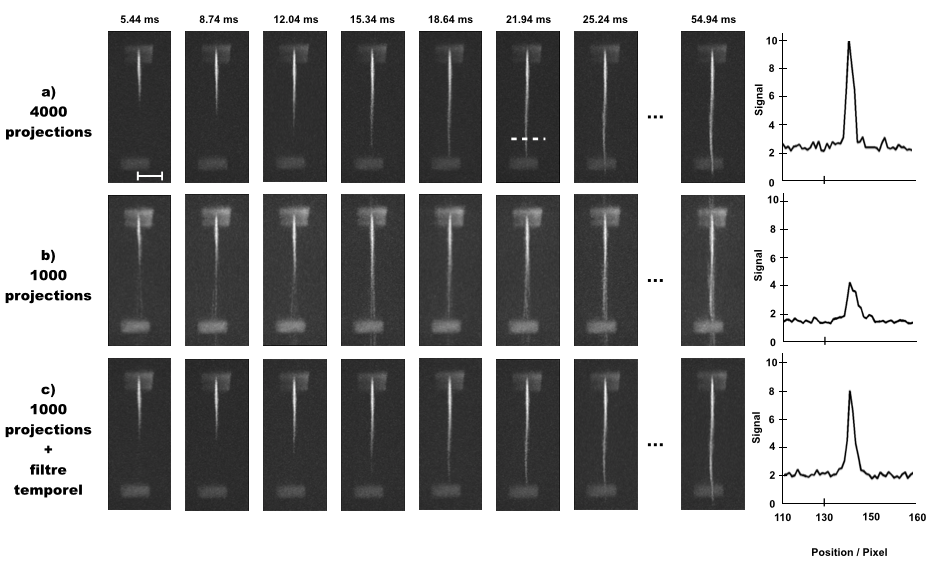
\includegraphics[scale=0.5]{./figure/chap3/ImFlowPhant.png}
\caption[Imagerie de flux dynamique in vitro.]{\label{fig:ImFlowPhant} \textbf{Imagerie de flux dynamique in vitro.} Images MIP coronales recueillies sur le fantôme de flux avec la séquence dynamique. Les images reconstruites avec (a) 4 000 ou (b) 1 000 projections sont comparées aux images reconstruites avec (c) 1 000 projections et l'utilisation d'un filtre temporel (R=3, Q=1). Le profil d'intensité est obtenu au niveau de la ligne en pointillée au temps 21,94 ms pour chaque cas. La barre d'échelle correspond à une longueur de 5 mm.}
\line(1,0){400} \\ \end{figure}

Les données sont sous-échantillonnées \textit{a posteriori} pour obtenir un jeu de données constitué de 1 000 et 4 000 projections correspondant respectivement à des temps d'acquisitions de 4 min 51 s et 1 min 13 s. Avec 4 000 projections (figure \ref{fig:ImFlowPhant}.a), il est possible de visualiser distinctement la progression du flux dans le tube et sa vitesse peut être correctement mesurée. La vitesse maximum observée est égale à 65 cm/s, ce qui correspond logiquement à 2 fois la valeur moyenne. Avec 1 000 projections (figure \ref{fig:ImFlowPhant}.b), on observe sur les images une nette infériorité en terme de signal et de résolution spatiale. Le signal sur bruit du tube passe de 10 à 4,2 entre 4 000 et 1 000 projections. On observe aussi la présence d'artefacts de streaking qui empêche la mesure d'une valeur précise de vitesse des flux. Cependant en utilisant le filtre temporel (R=3, Q=1) (figure \ref{fig:ImFlowPhant}.c) les artefacts de streaking sont supprimés et l'on observe que le profil de signal remonte de 4.2 à 8.
L'augmentation du volume de flux dans le champ de vue a été mesurée sur toutes les images ciné (correspondant à la progression du flux dans le tube) et l'on observe une sur-évaluation du volume sur les images reconstruites avec 1 000 projections (figure \ref{fig:GraphFlowPhant}). En revanche, avec l'utilisation du filtre on observe des données totalement en accord avec celles reconstruites avec 4 000 projections.

\begin{figure}[H]
\centering \line(1,0){400} \\
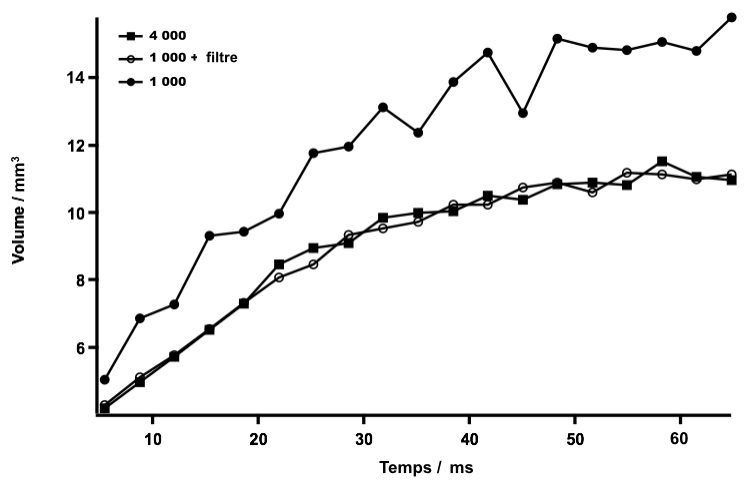
\includegraphics[scale=0.4]{./figure/chap3/GraphFlowPhant.png}
\caption[Quantification des flux in vitro en fonction du sous-échantillonnage.]{\label{fig:GraphFlowPhant} \textbf{Quantification des flux in vitro en fonction du sous-échantillonnage.} Volumes des flux mesurés en fonction du temps après l'application du module de saturation à partir des images obtenues sur fantôme. Les données représentées ont été recueillies avec 4 000, 1 000 et 1 000 + filtre des projections.}
\line(1,0){400} \\ \end{figure}

%\subsubsection{Imagerie in-vivo}
%
%Ces observations ont aussi été observé in-vivo sur les carotides de souris avec la même séquence synchronisée sur l'ECG. La comparaison des images non-filtrée et filtrée avec 1000, 2500 et 4000 projections (figure \ref{fig:ImFlowMice}) ainsi que les résultats de mesure de volume de flux (\ref{fig:GraphFlowMice}) montre qu'il est nécessaire d'utiliser un nombre de projection plus important in-vivo due à la qualité globale des images. Les images obtenue avec une reconstruction de 2500 projections et l'utilisation du filtre (R=3,Q=1) donne des résultats équivalent en terme de qualité d'image et de volume du flux. Dans la suite, nous utiliserons 2500 projections correspondant approximativement à 6 min 30 s de temps d'acquisition totale.
%\begin{figure}[H]
%\centering \line(1,0){400} \\
%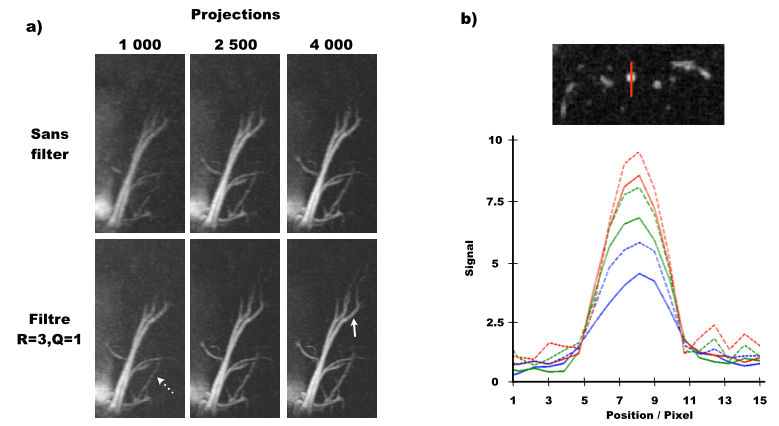
\includegraphics[scale=0.5]{./figure/chap3/ImFlowMice.png}
%\caption[Image ARM dynamique sur souris]{\label{fig:ImFlowMice} Images MIP sagital recueillies sur des carotides de souris avec la séquence dynamique. (a) Les images reconstruites avec 1000, 2500 et 4000 projections sont comparées aux images reconstruites avec l'utilisation d'un filtre temporel (R=3, Q=1). (b) Le profile d'intensité est obtenu au niveau de la ligne rouge sur les carotides après la bifurcation aortique. Lignes continues : reconstructions non-filtrées; bleu: 1000 projections; vert: 2500 projection; rouge: 4000 projections.}
%\line(1,0){400} \\ \end{figure}
%
%\begin{figure}[H]
%\centering \line(1,0){400} \\
%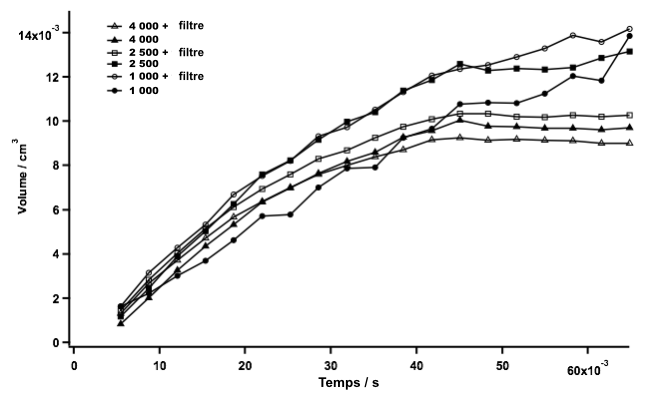
\includegraphics[scale=0.5]{./figure/chap3/GraphFlowMice.png}
%\caption[Graphique de progression du flux sur fantôme]{\label{fig:GraphFlowMice} Volume des flux mesuré en fonction du temps après l'application du module de saturation sur les carotides d'une souris saine. Les données représentées ont été recueillies avec 4000, 2500 et 1000 projections ainsi qu'avec leurs reconstruction filtrée (R=3,Q=1).}
%\line(1,0){400} \\ \end{figure}

\subsubsection{Imagerie du polygone de Willis}

%\begin{figure}[H]
%\centering \line(1,0){400} \\
%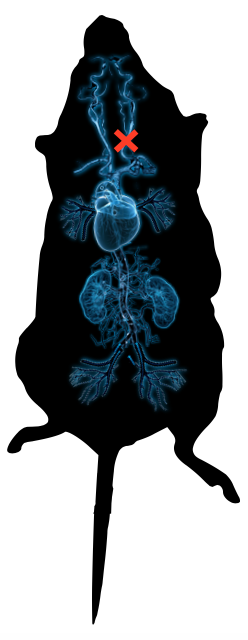
\includegraphics[scale=0.5]{./figure/chap3/LigatCarotide.png}
%\caption[Modèle de ligature des carotides]{\label{fig:LigatCarotide} Schéma du modèle de ligature de la carotide sur souris}
%\line(1,0){400} \\ \end{figure}

Des expériences ont ensuite été réalisées sur un modèle de souris normale et sur un modèle de souris présentant une ligature de la carotide commune. Des images ont été réalisées au niveau du polygone de Willis avec des résolutions spatiale et temporelle extrêmement élevées ($(156 \ \mu m)^3$ et 3,3 ms). 2 500 projections ont été utilisées pour chaque image ciné et les images reconstruites avec un filtre Q=1, R=3 sont montrées dans la figure \ref{fig:ImFlowWillis}. Les images ont été synchronisées sur le cycle cardiaque de l'animal. Le temps d'acquisition total est d'environ 5 minutes (avec 500 battements cardiaques par minute).

Avec la séquence d'ARM dynamique, il a été possible d'observer chez 4 souris ayant subi une ligature de la carotide droite (figure \ref{fig:ImFlowWillis}.a) que le remplissage du polygone était compensé par le flux sanguin provenant de la carotide gauche. Cependant le délai d'arrivée du sang dans la partie droite du polygone présente un retard par rapport aux souris contrôles comme observé sur les images de la figure \ref{fig:ImFlowWillis}.b.
Ce délai a pu être quantifié sur une carte paramétrique obtenue grâce à une méthode de calcul du temps d'arrivée du sang en un point de l'espace (figure \ref{fig:ColorMapFlowWillis}).

\begin{figure}[H]
\centering \line(1,0){400} \\
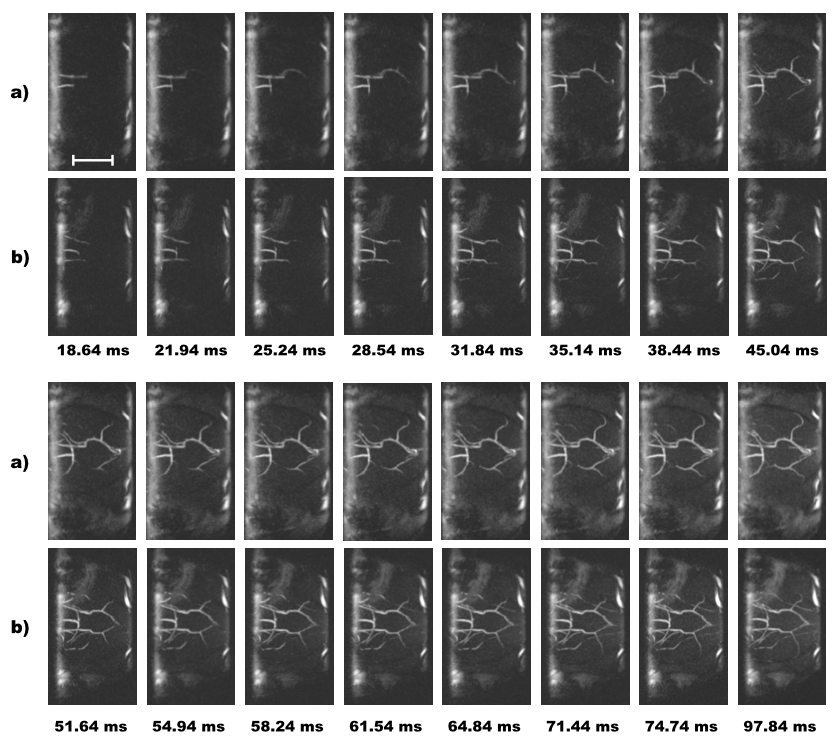
\includegraphics[scale=0.5]{./figure/chap3/ImFlowWillis.png}
\caption[Images d'ARM dynamique sur souris au niveau du polygone de Willis.]{\label{fig:ImFlowWillis} \textbf{Images d'ARM dynamique sur souris au niveau du polygone de Willis}. Images MIP d'ARM dynamique acquises sur une souris ayant subi une ligature d'une artère carotide (a) et sur une souris saine (b). 16 images ont été extraites sur les 30 images ciné acquises. La barre d'échelle représente 10 mm.}
\line(1,0){400} \\ \end{figure}

\begin{figure}[H]
\centering \line(1,0){400} \\
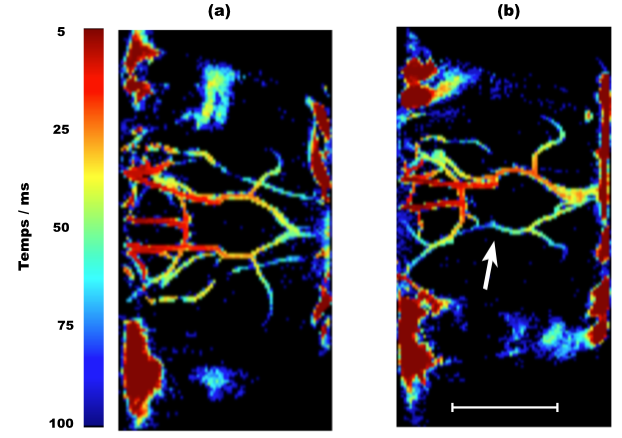
\includegraphics[scale=0.5]{./figure/chap3/ColorMapFlowWillis.png}
\caption[Quantification de la progression des flux sur une carte paramétrique.]{\label{fig:ColorMapFlowWillis} \textbf{Quantification de la progression des flux sur une carte paramétrique.} Carte paramétrique représentant le délai d'arrivée du sang dans une partie du polygone de Willis après saturation du volume imagé pour une souris saine (a) et pour une souris avec une artère carotide ligaturée (b). La barre d'échelle mesure 10 mm.}
\line(1,0){400} \\ \end{figure}

Il n'est pas possible d'effectuer l'imagerie sur un champ de vue plus large. En effet, le contraste vasculaire étant basé sur le principe du temps de vol, le signal sanguin sera saturé en arrivant à la fin du polygone. Une des solutions serait d'augmenter le TR de la séquence mais ceci entraînerait une moins bonne visualisation dynamique de l'avancée du flux. De plus, la différence entre deux images consécutives serait plus importante ce qui limiterait la taille du filtre temporel utilisable. Enfin un dernier problème se pose puisqu'il faudrait augmenter le nombre d'images ciné à lire après la saturation du signal ce qui induirait une repousse accrue du signal statique et donc diminuerait le contraste que l'on pourrait espérer obtenir entre le cerveaux et les vaisseaux.

L'alternative employée a été de répéter la séquence 3 fois de suite en modifiant la position du volume puis d'associer les images après leur reconstruction en fonction de leur position (figure \ref{fig:FluxComplet}.a). Les volumes sont disposés de manière à se superposer en partie pour limiter les effets de bord. On peut aussi reconstruire une carte paramétrique pour l'arrivée du flux mais cela demande à l'utilisateur d'indiquer à quel moment le flux d'un volume entre dans le suivante. La figure \ref{fig:FluxComplet}.b est un exemple de représentation en carte paramétrique utilisant de multiples volumes. On observe sur ces images des artefacts au bord des volumess qui sont dus à la mauvaise saturation du signal en bord de coupe.

\begin{figure}[H]
\centering \line(1,0){400} \\
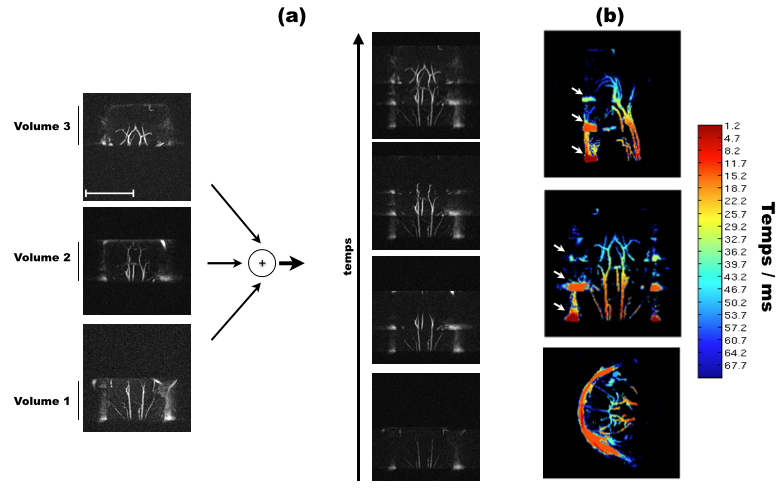
\includegraphics[scale=0.6]{./figure/chap3/FluxComplet.png}
\caption[Images d'ARM dynamique et carte paramétrique sur souris des carotides au niveau du polygone de Willis.]{\label{fig:FluxComplet} \textbf{Image d'ARM dynamique et carte paramétrique sur souris des carotides au polygone de Willis.} Imagerie des carotides jusqu'au polygone de Willis effectuée avec 3 acquisitions successives avec des coupes placées en 3 positions différentes. (a) L'association des images est effectuée après la reconstruction de chacune d'entre elles. (b) La carte paramétrique représentant l'avancée des flux doit être synchronisée pour que l'arrivée du sang dans la zone d'un premier volume débute en même temps que l'arrivée dans la même zone du volume d'imagerie suivant. La barre d'échelle mesure 10 mm.}
\line(1,0){400} \\ \end{figure}

\section{Discussion}

L'imagerie de flux chez la souris est un véritable défi du fait de la dimension des vaisseaux sanguins et des paramètres physiologiques extrêmes de la souris. Pour répondre à cette problèmatique, le développement d'une séquence radiale doublement pseudo-aléatoire a été préféré.

Dans un premier temps, une séquence avec une trajectoire 3D radiale projection-reconstruction pour l’ARM anatomique a été développée. Il a notamment été montré que cette méthode était beaucoup moins sensible aux artefacts de flux et de mouvement que l’imagerie cartésienne. Ceci a permis d’obtenir des images anatomiques de la crosse aortique avec un signal très homogène malgré la respiration et les flux turbulents durant la phase systolique du coeur. Ensuite, la capacité des méthodes radiales à être sous-échantillonnée a permis d’obtenir des images ayant une qualité satisfaisante avec seulement 4 000 projections. Ceci correspond à une réduction du temps d’acquisition d'un facteur supérieur à 14 par rapport au critère de Nyquist ainsi que de 10 par rapport à une séquence cartésienne standard permettant d’obtenir une imagerie avec le même champ-de-vue. 

Enfin, le troisième avantage de l’imagerie radiale mise en place ici est l’utilisation d’une trajectoire pseudo-aléatoire. Cela permet une distribution approximativement uniforme des projections au cours du temps. Cette méthode, peut être employée pour efficacement répartir les projections avec pour objectif de retirer les projections corrompues par les mouvements physiologiques. En effet, il existe des approches utilisant les points centraux des projections pour extraire des informations sur la position de celles-ci au sein de la respiration. Il peut donc être possible de reconstruire \textit{a posteriori} des images à différents moments de la phase de respiration, ou bien de reconstruire des images avec les projections recueillies uniquement durant les phases de respiration avec peu de mouvement. Cette méthode de correction de mouvement n’a pas été employée ici car les acquisitions chez la souris sont peu sensibles à ce type d’artefacts. En revanche, elle pourrait être pertinente pour une utilisation chez l’homme. Grâce à ces différents points, l’imagerie radiale utilisant une trajectoire d’angle d’or peut être particulièrement efficace pour l’imagerie anatomique temps-de-vol, en particulier si les temps d’acquisition ont besoin d’être limités ou sur des régions anatomiques sujettes aux mouvements.
 

Cette approche a ensuite été étendue à l'imagerie résolue dans le temps pour visualiser la progression des flux dans les vaisseaux avec une forte résolution temporelle (3,3 ms; 300 images/seconde), une forte résolution spatiale et surtout en un temps d'acquisition réduit d'un facteur 5 par rapport à la méthode précédemment employée par Miraux et al.
L'optimisation de la séquence permet d'obtenir des temps de répétition inférieurs à 3,5 ms qui sont nécessaires pour visualiser l'avancée des flux rapides dans les artères, cela est aussi important pour permettre l'utilisation du filtre temporel qui est plus efficace lorsqu'il existe peu de différence entre les images adjacentes.
L'utilisation du filtre temporel a été rendu possible grâce à l'ajout du second angle d'or entre les trajectoires des images ciné. Celui-ci a pour effet de particulièrement bien répartir les projections entre celles-ci et permet une utilisation optimale de nombreuses formes de filtre temporel comme les filtres linéaires \cite{Barger:2002fk}, KWIC \cite{Song2004Dynamic-MRI-wit}, exponentielles etc. Cela est particulièrement utile lorsque la dynamique des flux n'est pas connue ou potentiellement perturbée dans des modèles pathologiques. Dans ce cas, la résolution finale des images pourra être modulée pour obtenir des images avec une qualité adaptée à la quantification de la vitesse des flux.

\section{Limitations}

La méthode proposée présente tout de même certaines limitations :
\begin{itemize}
\item Pour obtenir un effet temps de vol efficace, il est important d’utiliser une coupe relativement fine. Ainsi, avec un encodage radial sphérique comme proposé ici, une grande partie du champ de vue est inutile. Notamment, chez l’homme, ou il est nécessaire d’utiliser des coupes très fines pour visualiser le polygone de willis (< 5 cm) le développement d’autres stratégies devra être envisagé pour utiliser l’imagerie radiale doublement aléatoire pour la mesure du flux sanguin. 
\item Une des difficultés de l’imagerie non-cartésienne est la nécessité de connaître parfaitement la trajectoire dans l’espace de Fourier. Il est donc nécessaire d’ajouter une preparation supplémentaire (mesure de la trajectoire) lors de l’acquisition des images. Ceci augmente le temps total d'expérience.
\item Il reste difficile de combiner reconstruction 3D non-cartésienne et méthode d’imagerie parallèle. Des publications récentes montrent que cela est possible, mais ces méthodes reste à évaluer (nuSpirit, compressed sensing, …)
\end{itemize}

\section{Perspectives}
\begin{itemize}
\item Pour le transfert de cette méthode chez l’homme, le développement des séquences de type Stack-Of-Stars est envisageable. Elles permettraient en effet de limiter le champ de vue dans la direction de coupe.

\item Afin d’accélérer encore la méthode proposée, une collaboration avec C Mistretta a débuté pour tester les méthodes de reconstruction de type HYPR (HighlY constrained back-PRojection). Ces dernières semblent particulièrement bien adaptées à notre stratégie qui génèrent un signal de fond très faible.
\end{itemize}

\cleardoublepage
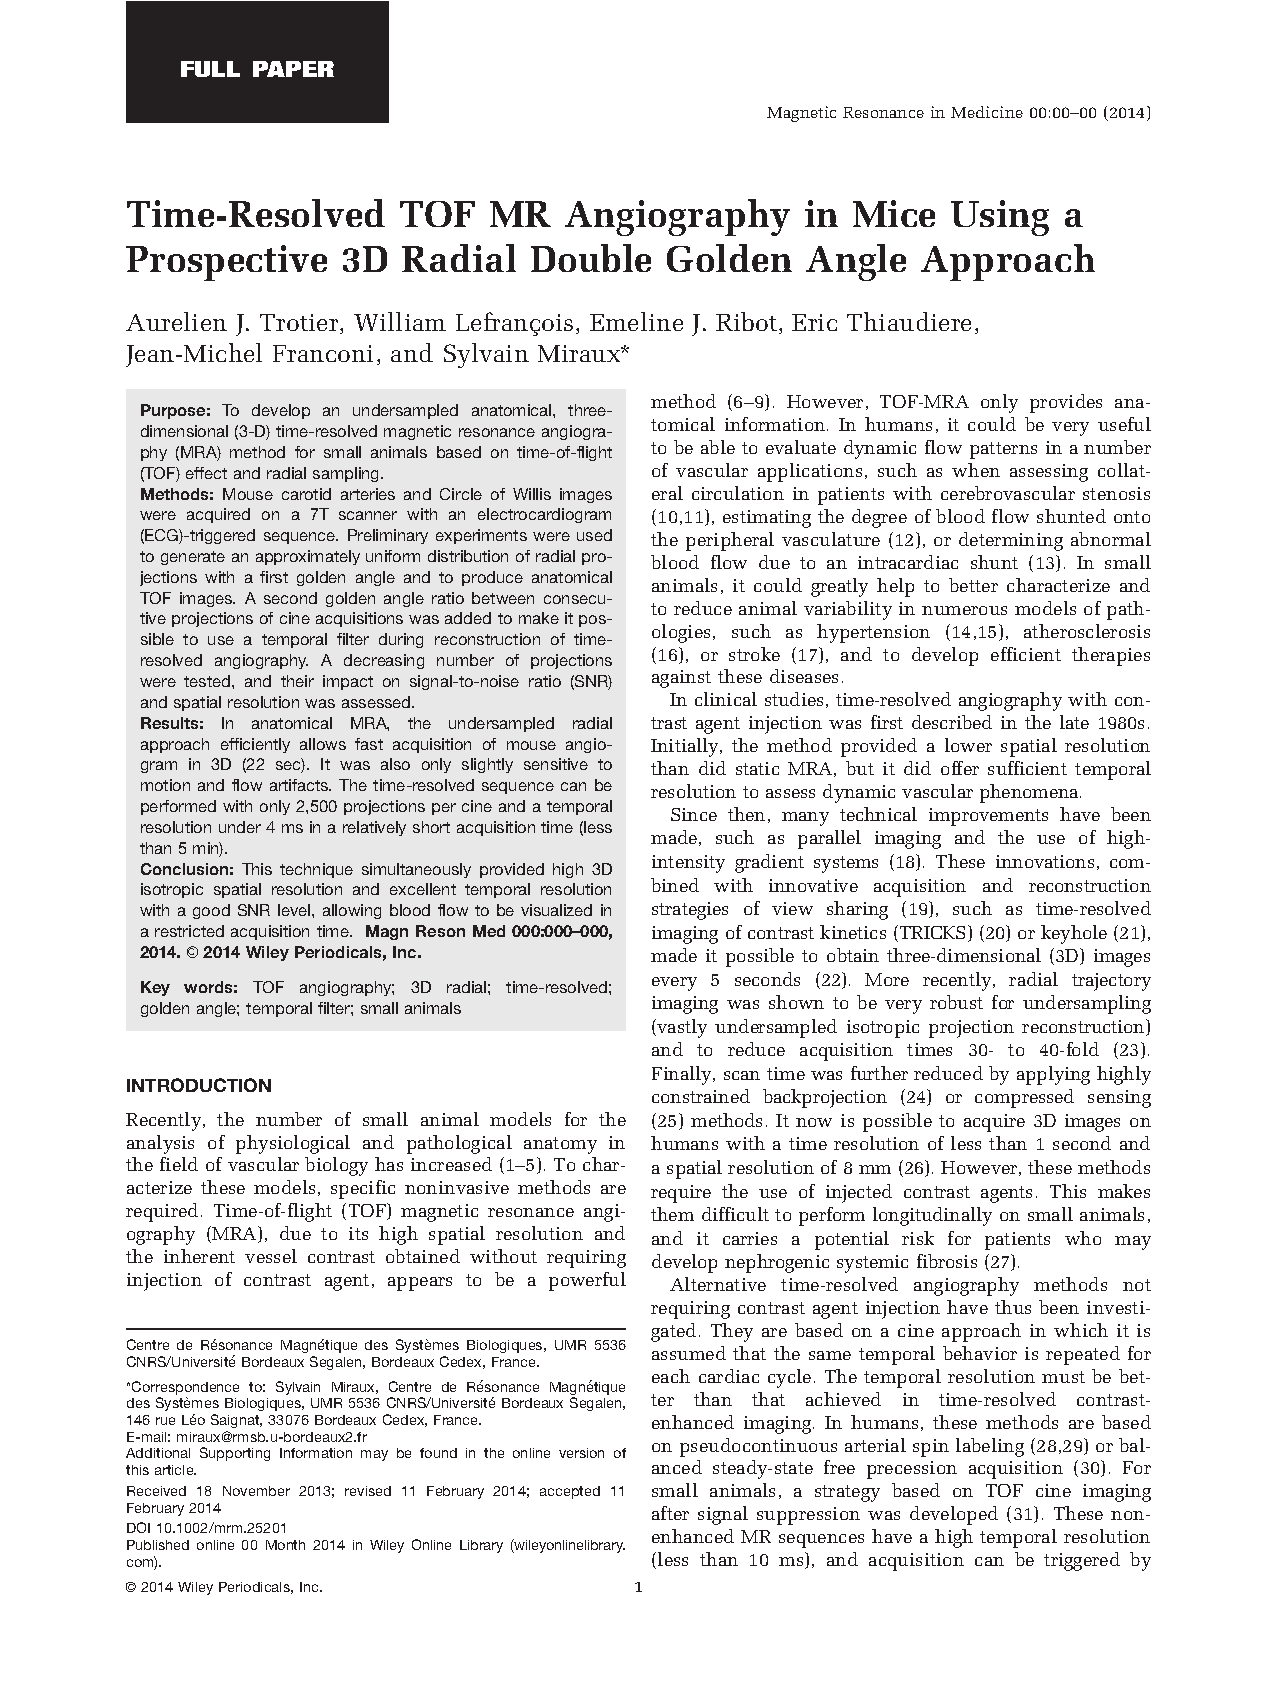
\includepdf[pages=1-11,pagecommand={\thispagestyle{plain}}]{./figure/chap3/Papier1.pdf}